% bei Standalone in documentclass noch:
% \RequirePackage{luatex85}

\documentclass[captions=tableheading, titlepage= firstiscover, parskip = half , bibliography=totoc]{scrartcl}
%paper = a5 für andere optinen
% titlepage= firstiscover
% bibliography=totoc für bibdateien
% parskip=half  Veränderung um Absätze zu verbessern

\usepackage{scrhack} % nach \documentclass
\usepackage[aux]{rerunfilecheck}
\usepackage{polyglossia}
\usepackage[style=numeric, backend=biber]{biblatex} % mit [style = alphabetic oder numeric] nach polyglossia
\addbibresource{lit.bib}
\setmainlanguage{german}

\usepackage[autostyle]{csquotes}
\usepackage{amsmath} % unverzichtbare Mathe-Befehle
\usepackage{amssymb} % viele Mathe-Symbole
\usepackage{mathtools} % Erweiterungen für amsmath
\usepackage{fontspec} % nach amssymb
% muss ins document: \usefonttheme{professionalfonts} % für Beamer Präsentationen
\usepackage{longtable}

\usepackage[
math-style=ISO,    % \
bold-style=ISO,    % |
sans-style=italic, % | ISO-Standard folgen
nabla=upright,     % |
partial=upright,   % /
]{unicode-math} % "Does exactly what it says on the tin."
\setmathfont{Latin Modern Math}
% \setmathfont{Tex Gyre Pagella Math} % alternativ

\usepackage[
% die folgenden 3 nur einschalten bei documenten
locale=DE,
separate-uncertainty=true, % Immer Fehler mit ±
per-mode=symbol-or-fraction, % m/s im Text, sonst \frac
]{siunitx}

% alternativ:
% per-mode=reciprocal, % m s^{-1}
% output-decimal-marker=., % . statt , für Dezimalzahlen

\usepackage[
version=4,
math-greek=default,
text-greek=default,
]{mhchem}

\usepackage[section, below]{placeins}
\usepackage{caption} % Captions schöner machen
\usepackage{graphicx}
\usepackage{grffile}
\usepackage{subcaption}

% \usepackage{showframe} Wenn man die Ramen sehen will

\usepackage{float}
\floatplacement{figure}{htbp}
\floatplacement{table}{htbp}

\usepackage{mhchem} %chemische Symbole Beispiel: \ce{^{227}_{90}Th+}


\usepackage{booktabs}

 \usepackage{microtype}
 \usepackage{xfrac}

 \usepackage{expl3}
 \usepackage{xparse}

 % \ExplSyntaxOn
 % \NewDocumentComman \I {}  %Befehl\I definieren, keine Argumente
 % {
 %    \symup{i}              %Ergebnis von \I
 % }
 % \ExplSyntaxOff

 \usepackage{pdflscape}
 \usepackage{mleftright}

 % Mit dem mathtools-Befehl \DeclarePairedDelimiter können Befehle erzeugen werden,
 % die Symbole um Ausdrücke setzen.
 % \DeclarePairedDelimiter{\abs}{\lvert}{\rvert}
 % \DeclarePairedDelimiter{\norm}{\lVert}{\rVert}
 % in Mathe:
 %\abs{x} \abs*{\frac{1}{x}}
 %\norm{\symbf{y}}

 % Für Physik IV und Quantenmechanik
 \DeclarePairedDelimiter{\bra}{\langle}{\rvert}
 \DeclarePairedDelimiter{\ket}{\lvert}{\rangle}
 % <name> <#arguments> <left> <right> <body>
 \DeclarePairedDelimiterX{\braket}[2]{\langle}{\rangle}{
 #1 \delimsize| #2
 }

\setlength{\delimitershortfall}{-1sp}

 \usepackage{tikz}
 \usepackage{tikz-feynman}

 \usepackage{csvsimple}
 % Tabellen mit \csvautobooktabular{"file"}
 % muss in table umgebung gesetzt werden


% \multicolumn{#Spalten}{Ausrichtung}{Inhalt}

\usepackage{hyperref}
\usepackage{bookmark}
\usepackage[shortcuts]{extdash} %nach hyperref, bookmark

\newcommand{\ua}[1]{_\symup{#1}}
\newcommand{\su}[1]{\symup{#1}}


\begin{document}

\section{Auswertung}

Im Folgendem werden die Messergebnisse ausgewertet und auf geeignete Weise
visualisiert.
Die verwendete Schaltung hatte die folgenden Daten.

\begin{align*}
  L &= \SI{3,53(3)}{\milli\henry} \\
  C &= \SI{5,015(15)}{\nano\farad} \\
  R_1 &= \SI{30,3(1)}{\ohm} \\
  R_2 &= \SI{271,6(3)}{\ohm}
\end{align*}

\subsection{Einhüllende der Schwingungskurve}

Die Wertepaare ($U_C(t_i), t_i$) müssen für die Ausgleichsrechnung bestimmt werden.
Die Werte $U_C(t_i)$ wurden mit dem Cursor des Oszilloskops gemessen.
Hingegen wurden die Zeiten $t_i$ aus dem Bild der Schwingungskurve mit
Hilfe eines Lineals abgelesen. Ein Abbild der Schwingungskurve ist in Abb.
\ref{fig:Schwingungskurve} dargestellt.

\begin{figure}
  \centering
  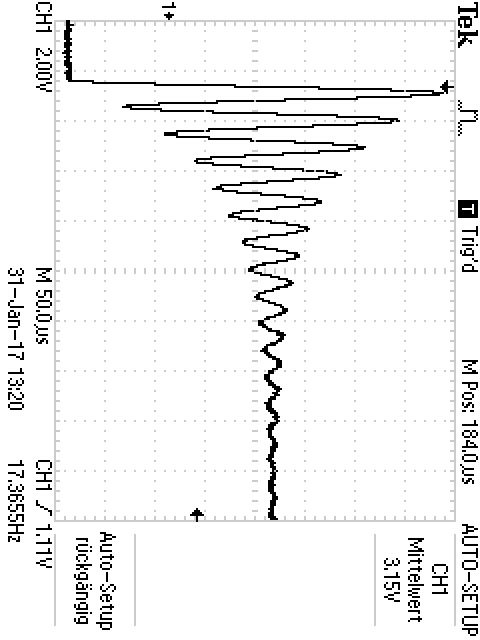
\includegraphics[width=\textwidth, angle=90, height=8cm]{F0001TEK.JPG}
  \caption{Gemessene Schwingungskurve.}
  \label{fig:Schwingungskurve}
\end{figure}

Die Schwingungskurve in Abb. \ref{fig:Schwingungskurve} wurde beim
Widerstand $R_1$ und einer Generatorfrequenz von $\SI{5,82}{\hertz}$ erstellt.

Die diskreten Wertepaare ($U_C(t_i), t_i$) sind in der Tabelle \ref{tab:Schwingungskurve}
dargestellt. Dabei wurden für $U_C(t_i)$ jeweils die Maxima der Schwingungskurve
vermessen.

\floatplacement{table}{htbp}
\begin{table}
 \centering
 \sisetup{table-format=3.2}
 \begin{tabular}[width=\textwidth]{S S}
     \toprule
      {Zeit in $\si{\micro\second}$} & {Maxima in $\si{\volt}$} \\
     \midrule
      0 & 15,08 \\
      27,5 & 13,2 \\
      55 & 11,92 \\
      82,5 & 10,96 \\
      112,5 & 10,24 \\
      142,5 & 9,68 \\
      172,5 & 9,36 \\
      202,5 & 9,04 \\
      235 & 8,88 \\
      267,5 & 8,76 \\
      302,5 & 8,64 \\
      337,5 & 8,52 \\
      \bottomrule
  \end{tabular}
  \caption{Messdaten der Schwingungskurve.}
  \label{tab:Schwingungskurve}
\end{table}

Mit den Wertepaaren aus Tabelle \ref{tab:Schwingungskurve} wurde mittels
des \emph{Python}-Paketes \emph{curve\_fit} eine Ausgleichsrechnung an eine
exponentielle Funktion der Form

\begin{align}
  \label{eqn:exp}
  U\ua{c}(t) = a\cdot\exp^{-b\cdot t} + c
\end{align}

durchgeführt. Für die Parameter ergeben sich somit die Werte

\begin{align*}
  a & = \SI{6,62(3)}{\volt} \\
  b &= \num{1,17(1)e4}\frac{1}{\si{\second}} \\
  c &= \SI{8,44(2)}{\volt}
\end{align*}

Die Ausgleichfunktion ist mit den Daten aus Tabelle \ref{tab:Schwingungskurve} in Abb. \ref{fig:Ausgleichsrechnung} dargestellt.

\floatplacement{table}{htbp}
\begin{figure}
  \centering
  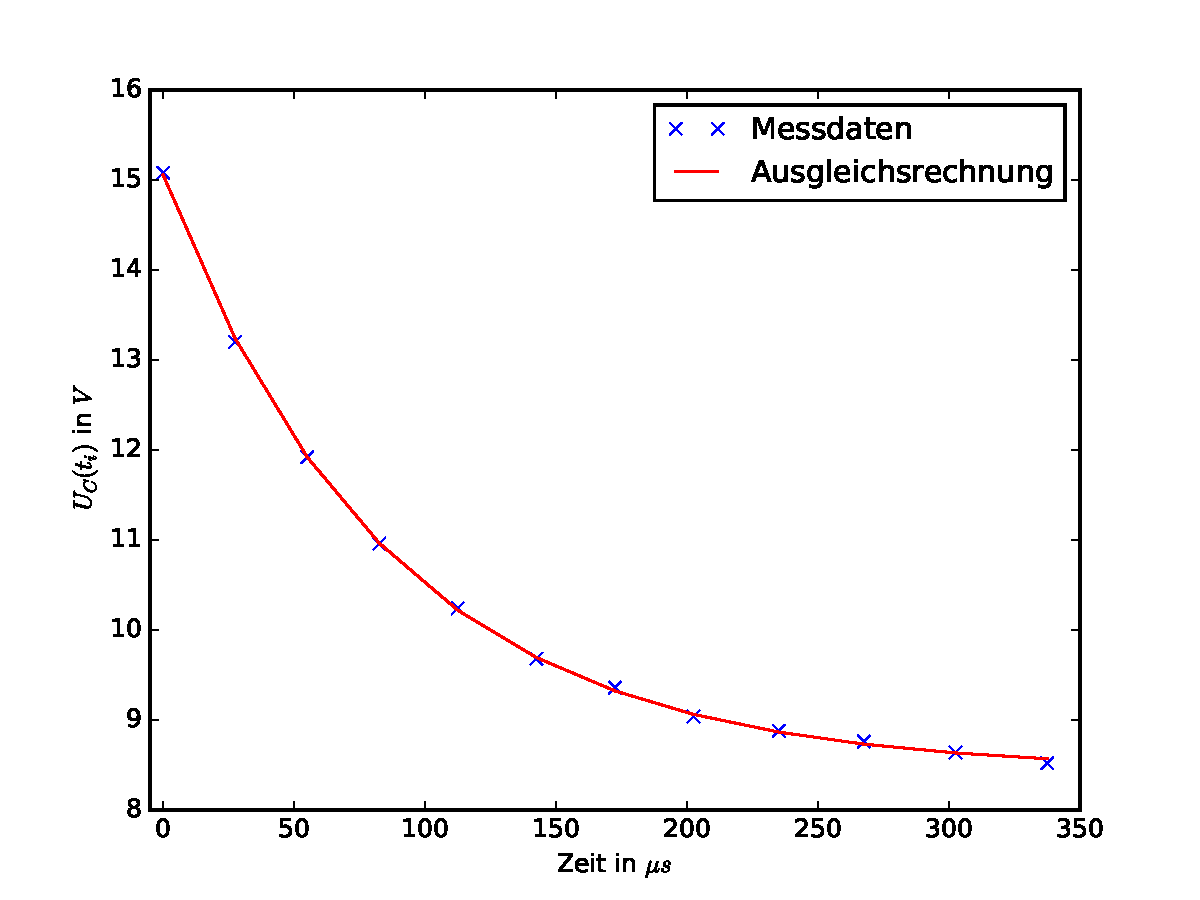
\includegraphics[width=\textwidth]{ausgleichsrechnung.pdf}
  \caption{Darstellung der Ausgleichsfunktion.}
  \label{fig:Ausgleichsrechnung}
\end{figure}

Der Exponent der Ausgleichsfunktion liefert über die Formeln (??) den
effektiv Widerstand $R\ua{eff}$ und die Abklingzeit $T\ua{ex}$.
Damit ergeben sich die folgenden Werte.

\begin{align*}
  R\ua{eff} &= \SI{82,4(12)}{\ohm}\\
  T\ua{ex} &= \SI{8,56(1)e-5}{\second}
\end{align*}

Im Vergleich zu dem eigebauten, verwendeten Widerstand $R_1$ fällt auf, dass
$R\ua{eff}$ deutlich größer ist. Dies ist damit zu begründen, dass $R\ua{eff}$
den Innenwiderstand des Generators mit einbezieht, welcher in $R_1$ nicht erfasst
wird.

\subsection{Widerstand im aperiodischen Grenzfall}

Aus den Daten $L$ und $C$ der Apparatur lässt sich über Formel (??) der
Widerstand des aperiodischen Grenzfalles $R\ua{ap}$ errechnen.
Der Wert $R\ua{ap}$ wurde auch experimentell bestimmt. Die Messung ergeben
die folgenden Werte.

\begin{align*}
  R\ua{ap,theo} = \SI{1678(8)}{\ohm}
  R\ua{ap} = \SI{13500}{\ohm}
\end{align*}

Die Messung wurde bei einer Frequenz von $\nu = \SI{5,82}{\hertz}$ erhoben.
Der Wert $R\ua{ap}$ ist der experimentell bestimmte Wert. Dieser wurde an
dem variablen Widerstand der Apparatur abgelesen und wird als fehlerfrei
angenommen. Die gemessene Wert ist ca. acht mal größer als der
theoretisch berechnete Wert. Dies hängt damit zusammen, dass der experimentelle
Wert an der Apparatur nur ungenau abzulesen war. Zudem war nicht sichergestellt,
dass der abgelesene Widerstand tatsächlich mit dem angelegten Widerstand
übereinstimmt. Damit ist die Diskrepantz auf einen systematischen
Fehler zurückzuführen.

\subsection{Resonanzfrequenz}

Die Resonanzfrequenz lässt sich mit den Apparaturdaten über die Formel (??)
errechnen. Als Widerstand wurde der gemessene effektiv Widerstand $R\ua{eff}$
verwendet.
Die berechnete Resonanzfrequenz beträgt:

\begin{align*}
  \nu\ua{res} &= \SI{3.774(17)e4}{\hertz}.
\end{align*}

In dem Diagramm \ref{fig:Kondensator_Frequ} ist die normierte Kondensatorspannung
in Abhängigkeit von der Frequenz dargestellt. Mit normiert ist gemeint, dass die
Kondensatorspannung durch die Generatorspannung geteilt wird.
Das Diagramm \ref{fig:Kondensator_Frequ} wurde mit den Daten aus Tabelle \ref{tab:Kondensator_Frequ}
erstellt.

\floatplacement{table}{htbp}
\begin{figure}
  \centering
  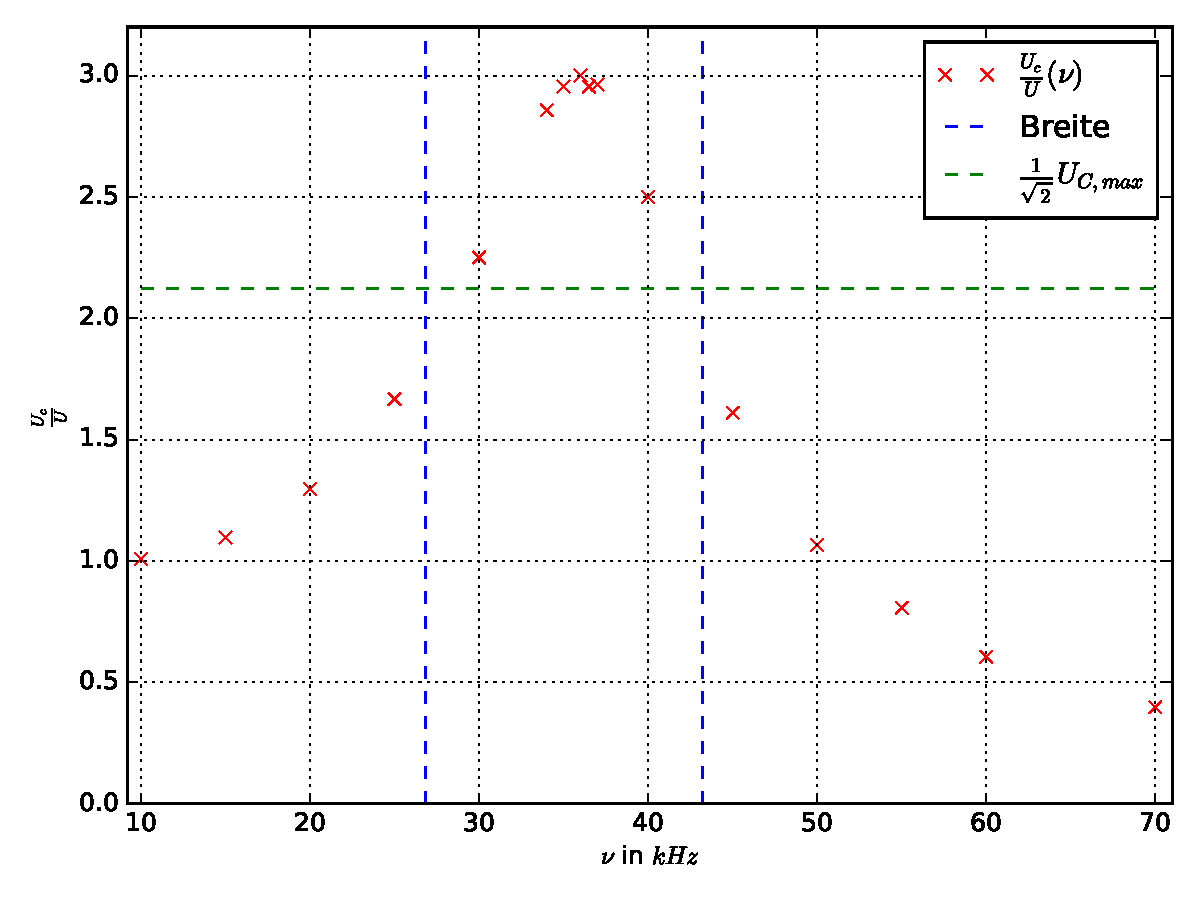
\includegraphics[width=\textwidth]{messung_c.pdf}
  \caption{Normierte Kondensatorspannung in Abhängigkeit von der Frequenz.}
  \label{fig:Kondensator_Frequ}
\end{figure}

Der Maximalwert der Kondensatorspannung wird bei einer Frequenz von

\begin{equation}
  \label{eqn:Resonanzfrequenz}
  \nu\ua{res} = \SI{36}{\kilo\hertz}
\end{equation}

gemessen. Die Halbwertsbreite der Kondensatorspannung ist durch die Differenz der Werte
$\nu_+$ und $\nu_-$ gegeben.

\begin{align*}
  \nu_+ &\approx \SI{27}{\kilo\hertz} \\
  \nu_- &\approx \SI{43}{\kilo\hertz}
\end{align*}

Damit ergibt sich die Breite zu $\approx 16\si{\kilo\hertz}$.

Die dazugehörigen Theoriewerte lassen sich über \eqref{} errechnen.

\begin{align*}
  \nu\ua{+,theo} &= \SI{23,32(27)}{\kilo\hertz} \\
  \nu\ua{-,theo} &= \SI{46,7(5)}{\kilo\hertz}
\end{align*}

Die Werte weichen nur geringfügig voneinander ab.
Die Güte $q$ des Schwingkreises ist der Maximalwert des Verhältnises von
Kondensatorspannung zur Generatorspannung.
In Abb. \ref{fig:Kondensator_Frequ} ist das Maximalverhältnis bei der
Resonanzfrequenz erreicht. An diesem Punkt beträgt das Verhältnis

\begin{equation*}
  q = 3.
\end{equation*}

Der errechnete Wert liegt bei $q\ua{theo} = 3,24$ und stimmt im Rahmen der
Messungenauigkeiten mit dem gemessenen Wert überein.

\subsubsection{Resonanzfrequenz aus der Phasenverschiebung}

Aus der Phasenverschiebung zwischen Generator- und Kondensatorspannung in Abhängigkeit
von der Frequenz kann die Resonanzfrequenz $\nu\ua{res}$ bestimmt werden.
Die Resonanzfrequenz ist der Wert, an dem die Phase zwischen den Spannungen
$\varphi\ua{res} = \frac{\pi}{2}$ entspricht.
Der gemessene Wert wurde aus dem Diagramm \ref{fig:Resonanz} abgelesen.

\floatplacement{table}{htbp}
\begin{figure}
  \centering
  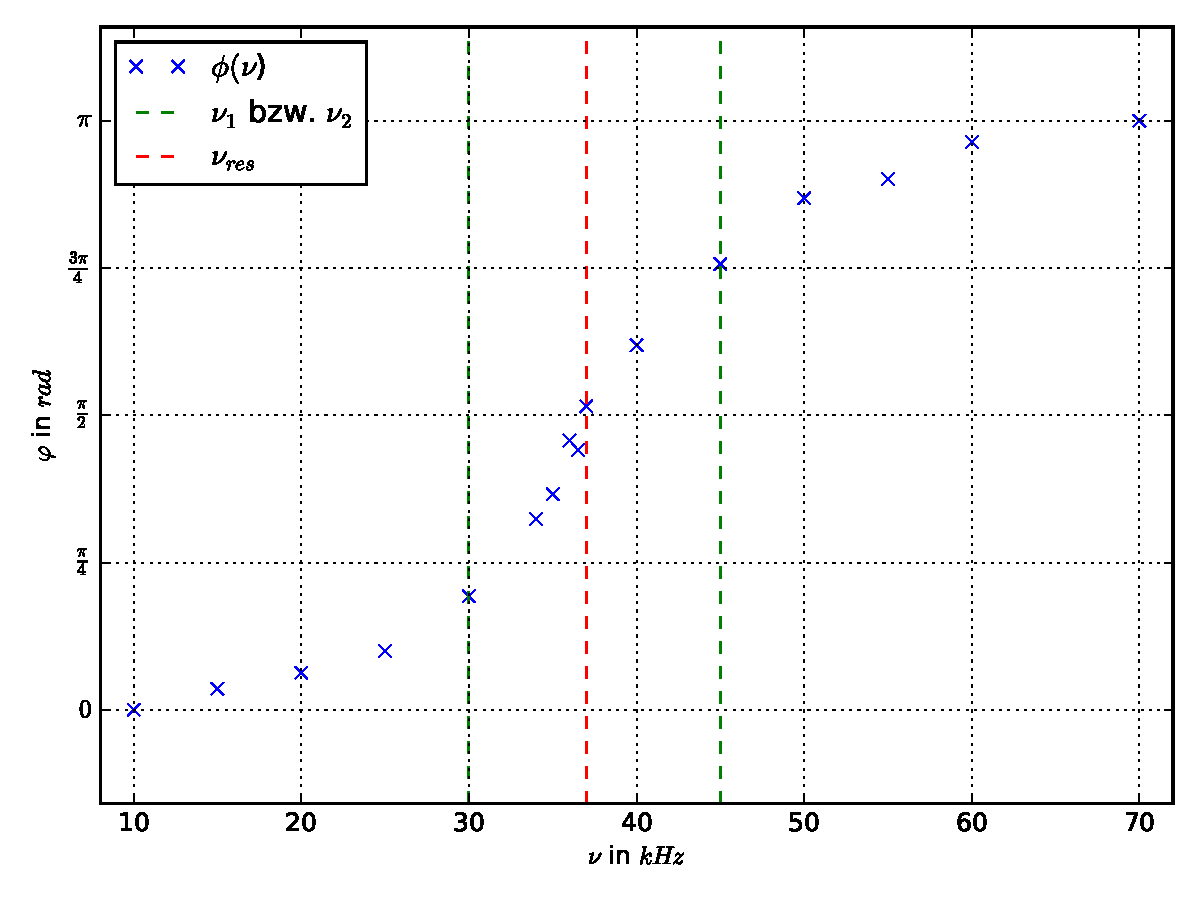
\includegraphics[width=\textwidth]{phase_gegen_nu.pdf}
  \caption{Phase zwischen Kondensator- und Generatorspannung in Abhängigkeit von der Frequenz.}
  \label{fig:Resonanz}
\end{figure}

Der abgelesene Wert bei einer Phase von $\varphi\ua{res}$ ist:

\begin{equation*}
  \nu\ua{res} = \SI{37}{\kilo\hertz}.
\end{equation*}

Dieser Wert stimmt mit dem berechneten und in \eqref{eqn:Resonanzfrequenz} bestimmten
Wert nahezu überein.

Die Frequenz $\nu_1$, bei der die Freqeunz gerade $\frac{\pi}{4}$ ist, sowie die
Frequenz $\nu_2$, bei der $\varphi = \frac{3\pi}{4}$ ist sind dem Diagramm \ref{fig:Resonanz}
näherungsweise zu entnehmen.

\begin{align*}
  \nu_1 &\approx \SI{30}{\kilo\hertz} \\
  \nu_2 &\approx \SI{45}{\kilo\hertz}
\end{align*}

Rechnerisch ergeben sich über die Formel \eqref{??} $\nu_1$ und $\nu_2$ zu:

\begin{align*}
  \nu\ua{1,theo} &= \SI{36,21(17)}{\kilo\hertz} \\
  \nu\ua{2,theo} &= \SI{38,55(17)}{\kilo\hertz}
\end{align*}

Die Werte weichen deutlich von den gemessenen Werten ab.
Dies ist damit zu begründen, dass die gemessenen Werte nur Näherungen entsprechen.
Damit eine höhere Sicherheit der Messdaten besteht, hätten mehr Messwerte um den
Bereich einer Phasenverschiebung von $\varphi = \frac{\pi}{4}$ bzw.
$\varphi = \frac{3\pi}{4}$ genommen werden müssen. Es lässt sich aufgrund der
mangelnden Anzahl an Messwerten keine präzise Begründung für die signifikanten Unterschiede
zwischen den Theoriewerten und den gemessenen Werten machen.

\section{Diskussion}

Anhand der ausgewerteten Daten wird deutlich, dass lediglich der gemessene
Widerstand des aperiodischen Grenzfalles enorm vob dem theoretisch berechneten Wert
abweicht.
Die aufgetretene Abweichnung wurde auf einen systematischen Fehler zurückgeführt.
Zudem weichen die bestimmten Frequenzen $\nu_1$ und $\nu_2$ deutlich von den
berechneten Werten ab. Dies wurde mit der geringfügigen Aussagekraft der wenigen
Messdaten in den Bereich von $\varphi = \frac{\pi}{4}$ und $\varphi = \frac{3\pi}{4}$
begründet.
Die sonstigen Werte entsprachen alle im Rahmen der Messungenauigkeiten den theoretisch
berechneten Werten.

\section{Messdaten}

Die Daten der Messung zur Resonanzfrequenz sind in der folgenden Tabelle dargestellt.

\floatplacement{table}{htbp}
\begin{table}
 \centering
 \sisetup{table-format=2.1}
 \begin{tabular}[width=\textwidth]{S S S S S}
     \toprule
      {$\nu_G$ in $\si{\kilo\hertz}$} & {$\lambda$ in $\si{\micro\second}$} & {$\varphi$ in $\si{\micro\second}$} & {$U\ua{G}$ in $\si{\volt}$} & {$U\ua{C}$ in $\si{\volt}$} \\
     \midrule
      10 & 98,0 &   0    &  5,4  & 5,4 \\
      15 & 67,0 &   1,2  &  5,4  & 5,9 \\
      20 & 50,8 &   1,6  &  5,1  & 6,6 \\
      25 & 40,0 &   2,0  &  5,0  & 8,4 \\
      30 & 33,2 &   3,2  &  4,8  & 10,8 \\
      34 & 29,6 &   4,8  &  4,5  & 12,8 \\
      35 & 28,4 &   5,2  &  4,4  & 13,0 \\
      36 & 28,0 &   6,4  &  4,4  & 13,2 \\
      36,5&27,2 & 6,0  &  4,4  & 13,0 \\
      37 & 26,4 &   6,8  &  4,3  & 12,8 \\
      40 & 25,2 &   7,8  &  4,5  & 11,2 \\
      45 & 22,2 &   8,4  &  4,7  & 7,6 \\
      50 & 19,8 &   8,6  &  4,9  & 5,2 \\
      55 & 18,2 &   8,2  &  5,0  & 4,0 \\
      60 & 16,6 &   8.0  &  5,0  & 3,0 \\
      70 & 14,0 &   7.0  &  5,0  & 2,0 \\
      \bottomrule
  \end{tabular}
  \caption{Messdaten zur Resonanzfrequenz.}
  \label{tab:Kondensator_Frequ}
\end{table}

\end{document}
